\section{Accuracy under skipping}\label{app:accuracy}

The change-rate certificate bounds accuracy only through $\kappa\alpha$, which can exceed a helpful path's gain. However, gold labels on a few skipped disagreements bound the loss directly: skipping can lower accuracy only on skipped questions where the reference is correct and the receiver alone is wrong. At $\alpha=0.05$, the three large-pair Text policies retain 33 to 105\% of the reference's gain. Stricter tolerances ($\alpha\le0.03$), which require labels to set, retain more gain on OBQA, ARC, and Text+fact, though not on MMLU-Pro.

\paragraph{Gain retention.} Under rules fixed before computing, we measured the reference's gain over the receiver ($G=\mathrm{acc}(b)-\mathrm{acc}(R)$), the policy's gain ($\mathrm{acc}(\pi_\tau)-\mathrm{acc}(R)$), and the share of $G$ retained, using paired bootstrap intervals. We repeated the certification with $\alpha$ from 0.01 to 0.05 at the same per-candidate cutoff (Table~\ref{tab:retention}; Figure~\ref{fig:corrections}b). At $\alpha=0.05$, policies retain 0.750 [0.467, 1.067] of Text's gain on OBQA, 1.054 [0.717, 1.858] on MMLU-Pro, and 0.333 [$-1.0$, 1.4] on ARC, where the gain itself is uncertain ($G=2.01$ points [$-0.33$, $+4.68$]; $G\le0$ in 6.8\% of resamples), and Text+fact retains 0.811 [0.686, 0.927]. On the 744 held-out OBQA questions, where $R$ ran on every question, large Text retains 0.759 [0.500, 0.958] and Text+fact retains 0.817 [0.706, 0.933]; the sealed ARC run did not execute $R$ on routed questions. The largest $\alpha$ with $\kappa\alpha<G$ is 0.04 for OBQA/Text (threshold deployed at 0.05), 0.02 for ARC/Text, 0.03 for MMLU-Pro/Text, and 0.05 for Text+fact; any such $\alpha$ must be chosen with labels. For these thresholds, we recomposed the panel saving from the per-request timings of each existing replay, excluding cold requests: a question the stricter policy still skips retains its recorded policy latency, and a routed question is charged its recorded probe latency plus the fixed arm's latency on that question; at the original thresholds this reproduces the measured saving within 1~ms. The recomposed savings are 532.9, 587.3, and 247.0~ms on the original configuration and 420.3 to 429.5, 469.3 to 479.5, and 197.1 to 199.8~ms in the three repeats on the second one (OBQA, ARC, and MMLU-Pro), and 342.7~ms for Text+fact on the second configuration; these are not new replays.

\paragraph{Lost reference corrections.} On skipped questions a policy replaces the reference's answer by the receiver's own, so for the skip set $O_\tau=\{x:s(x)\le\tau\}$ and gold label $y$, $\mathrm{acc}(\pi_\tau)-\mathrm{acc}(b)=\Pr(x\in O_\tau,\,o_R=y,\,o_b\neq y)-\Pr(x\in O_\tau,\,o_R\neq y,\,o_b=y)$: the receiver's successes that skipping recovers minus the reference corrections (questions the reference answers correctly and $R$ does not) that it loses. The identity holds in all fourteen OBQA, ARC, and large-pair MMLU-Pro settings. No C2C policy loses more than 3 reference corrections, whereas large/OBQA/Text loses 13 of 46 and large/ARC/Text 6 of 10 (Figure~\ref{fig:corrections}a); net of the successes they recover, the C2C policies answer 1 to 24 more questions correctly than their references, large/MMLU-Pro/Text answers 2 more, and large/OBQA/Text and large/ARC/Text answer 7 and 4 fewer. These are descriptive development outcomes that the risk test does not target. Questions where some action is correct but the policy is not (unused three-action opportunity) are more common on the kept side in seven of the eight settings; this does not show that the probe identifies them or that a three-action router could realize the oracle.

\begin{figure}[!t]\centering
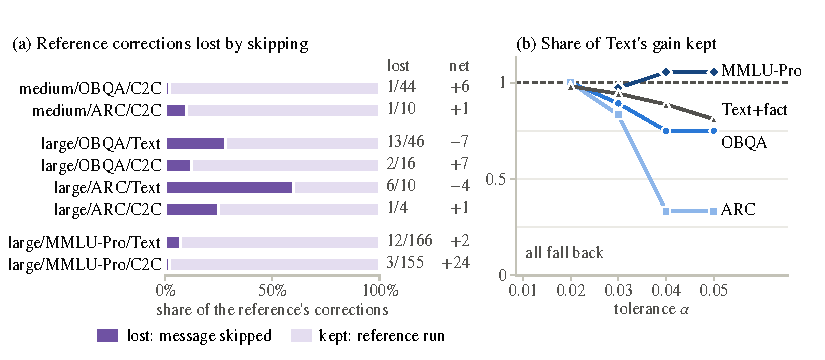
\includegraphics[width=\linewidth]{figures/figure_corrections.pdf}
\caption{Skipping loses few reference corrections under C2C but more under Text, and a stricter tolerance keeps more of Text's gain except on MMLU-Pro. (a)~Reference corrections (development questions the reference answers correctly and the receiver alone does not) that each deployed Qwen-pair policy loses by skipping or keeps by running the reference, with the lost count out of all the reference's corrections and the net change in correct answers (policy minus reference, gained minus lost). (b)~Share of the reference's gain over the receiver that the large-pair Text policies keep at each tolerance $\alpha$ (Table~\ref{tab:retention}); missing points fall back, and the dashed line marks the whole gain. Development populations; descriptive and gold-dependent; large/OBQA/Text, large/OBQA/C2C, and Text+fact are nominal (Appendix~\ref{app:history}).}
\label{fig:corrections}
\end{figure}

\begin{table}[!htbp]\centering\scriptsize
\caption{Lowering $\alpha$ never raises coverage; at $\alpha\le0.03$ it keeps more of the reference's gain over the receiver on OBQA, ARC, and Text+fact, but not on MMLU-Pro (development sets). $q$: deployed quantile (fallback: no threshold passes; --: not applicable). Changed: changed/skipped development questions. $\kappa\alpha$: worst-case accuracy loss (points). Retained: share of $G$ kept; $G$ is 3.77 (OBQA), 2.01 (ARC), 1.40 (MMLU-Pro), and 7.14 points (Text+fact).}
\label{tab:retention}
\renewcommand{\arraystretch}{1.1}\setlength{\tabcolsep}{3pt}
\begin{tabular}{lcccccc@{\hspace{10pt}}cccccc}\toprule
& \multicolumn{5}{c}{large/OBQA/Text} & & \multicolumn{5}{c}{large/ARC/Text}\\\cmidrule(lr){2-6}\cmidrule(lr){8-12}
\multicolumn{1}{c}{$\alpha$} & $q$ & Coverage (\%) & Changed & $\kappa\alpha$ & Retained & & $q$ & Coverage (\%) & Changed & $\kappa\alpha$ & Retained\\\midrule
0.01 & fallback & 0 & -- & -- & -- & & fallback & 0 & -- & -- & --\\
0.02 & 0.65 & 62.0 & 6/460 & 1.24 & 1.000 & & 0.80 & 77.9 & 0/233 & 1.56 & 1.000\\
0.03 & 0.75 & 72.2 & 15/536 & 2.17 & 0.893 & & 0.85 & 84.9 & 1/254 & 2.55 & 0.833\\
0.04 & 0.80 & 77.1 & 19/572 & 3.08 & 0.750 & & 0.95 & 95.0 & 9/284 & 3.80 & 0.333\\
0.05 & 0.80 & 77.1 & 19/572 & 3.85 & 0.750 & & 0.95 & 95.0 & 9/284 & 4.75 & 0.333\\\midrule
& \multicolumn{5}{c}{large/MMLU-Pro/Text} & & \multicolumn{5}{c}{large/OBQA/Text+fact}\\\cmidrule(lr){2-6}\cmidrule(lr){8-12}
0.01 & fallback & 0 & -- & -- & -- & & fallback & 0 & -- & -- & --\\
0.02 & fallback & 0 & -- & -- & -- & & 0.55 & 53.6 & 1/398 & 1.07 & 0.981\\
0.03 & 0.30 & 30.7 & 16/812 & 0.92 & 0.973 & & 0.65 & 62.0 & 3/460 & 1.86 & 0.943\\
0.04 & 0.35 & 36.0 & 31/952 & 1.44 & 1.054 & & 0.70 & 66.4 & 7/493 & 2.66 & 0.887\\
0.05 & 0.40 & 40.5 & 40/1069 & 2.02 & 1.054 & & 0.75 & 72.2 & 13/536 & 3.61 & 0.811\\\bottomrule
\end{tabular}
\end{table}

\begin{table}[!htbp]\centering\scriptsize
\caption{The lost-correction test needs gold labels only on the calibration disagreements up to its first rejected candidate or the deployed threshold, whichever is lower ($D_{\rm need}$), and at $\varepsilon=0.01$ it is infeasible on the two ARC settings. Lost-correction test: exact binomial test of $H_0$: rate of lost corrections (skipped questions the reference gets right and $R$ wrong) $\ge\varepsilon$, the certified accuracy-loss bound. Accepted: candidates (of 20) accepted by the lost-correction test, the change-rate test, and both. $q_L$: largest candidate the lost-correction test accepts; $q_{\rm joint}$: largest candidate both accept (deployed by the joint certificate); $N$: calibration questions; infeasible: $N$ below the 688 that $\varepsilon=0.01$ needs. Disagreements: all ($D_{\rm all}$), up to the first rejected candidate ($D_{\rm seq}$), at $q_{\rm joint}$ ($D_{\rm dep}$), and up to that candidate or the deployed threshold, whichever is lower ($D_{\rm need}$). Without reviewed: $q_{\rm joint}$ without the parser-review questions (1,158 OBQA and 315 ARC remain; infeasible: 315 is below the 342 that $\varepsilon=0.02$ needs); parser-review questions: 341 calibration questions whose outputs were read with gold labels before the parser was frozen. --: not applicable. $^\ddagger$Nominal certificate.}
\label{tab:lostcal}
\renewcommand{\arraystretch}{1.1}\setlength{\tabcolsep}{2.5pt}
\vspace{5pt}\textit{(a) Accepted candidates and certified thresholds}\par\smallskip
\begin{tabular*}{\linewidth}{@{}l@{\hspace{5pt}\extracolsep{\fill}}ccccccccc@{}}\toprule
& & & \multicolumn{3}{c}{Candidates accepted (of 20)} & \multicolumn{3}{c}{Largest accepted $q$} & \\\cmidrule(lr){4-6}\cmidrule(lr){7-9}
Setting & $\varepsilon$ & $N$ & \begin{tabular}[b]{@{}c@{}}lost-\\correction\end{tabular} & \begin{tabular}[b]{@{}c@{}}change-\\rate\end{tabular} & both & \begin{tabular}[b]{@{}c@{}}lost-correction\\($q_L$)\end{tabular} & \begin{tabular}[b]{@{}c@{}}both\\($q_{\rm joint}$)\end{tabular} & \begin{tabular}[b]{@{}c@{}}change-rate\\(deployed)\end{tabular} & \begin{tabular}[b]{@{}c@{}}$q_{\rm joint}$ without\\reviewed\end{tabular}\\\midrule
large/OBQA/Text$^\ddagger$ & 0.01 & 1,366 & 13 & 16 & 13 & 0.65 & 0.65 & 0.80 & 0.60\\
large/OBQA/Text$^\ddagger$ & 0.02 & 1,366 & 15 & 16 & 15 & 0.75 & 0.75 & 0.80 & 0.75\\
\addlinespace[2pt]
large/ARC/Text & 0.01 & 448 & 0 & 19 & 0 & infeasible & infeasible & 0.95 & infeasible\\
large/ARC/Text & 0.02 & 448 & 16 & 19 & 16 & 0.80 & 0.80 & 0.95 & infeasible\\
\addlinespace[2pt]
large/MMLU-Pro/Text & 0.01 & 6,000 & 9 & 8 & 8 & 0.45 & 0.40 & 0.40 & 0.40\\
large/MMLU-Pro/Text & 0.02 & 6,000 & 12 & 8 & 8 & 0.60 & 0.40 & 0.40 & 0.40\\
\addlinespace[2pt]
large/OBQA/Text+fact$^\ddagger$ & 0.01 & 1,366 & 11 & 15 & 11 & 0.55 & 0.55 & 0.75 & 0.55\\
large/OBQA/Text+fact$^\ddagger$ & 0.02 & 1,366 & 14 & 15 & 14 & 0.70 & 0.70 & 0.75 & 0.65\\
\addlinespace[2pt]
Llama-8B/OBQA/Text & 0.01 & 1,366 & 9 & 10 & 7 & 0.45 & 0.45 & 0.60 & 0.35\\
Llama-8B/OBQA/Text & 0.02 & 1,366 & 12 & 10 & 10 & 0.60 & 0.60 & 0.60 & 0.50\\
\addlinespace[2pt]
Llama-8B/ARC/Text & 0.01 & 448 & 0 & 8 & 0 & infeasible & infeasible & 0.70 & infeasible\\
Llama-8B/ARC/Text & 0.02 & 448 & 9 & 8 & 3 & 0.45 & 0.45 & 0.70 & infeasible\\\bottomrule
\end{tabular*}
\par\vspace{17pt}
\textit{(b) Calibration disagreements that need gold labels}\par\smallskip
\begin{tabular*}{\linewidth}{@{}l@{\hspace{5pt}\extracolsep{\fill}}ccccc@{}}\toprule
& & \multicolumn{4}{c}{Calibration disagreements}\\\cmidrule(l){3-6}
Setting & $\varepsilon$ & all ($D_{\rm all}$) & up to the first rejection ($D_{\rm seq}$) & at $q_{\rm joint}$ ($D_{\rm dep}$) & labels needed ($D_{\rm need}$)\\\midrule
large/OBQA/Text$^\ddagger$ & 0.01 & 143 & 8 & 4 & 8\\
large/OBQA/Text$^\ddagger$ & 0.02 & 143 & 18 & 12 & 18\\
\addlinespace[2pt]
large/ARC/Text & 0.01 & 12 & 0 & -- & 0\\
large/ARC/Text & 0.02 & 12 & 1 & 0 & 1\\
\addlinespace[2pt]
large/MMLU-Pro/Text & 0.01 & 1,295 & 153 & 67 & 67\\
large/MMLU-Pro/Text & 0.02 & 1,295 & 361 & 67 & 67\\
\addlinespace[2pt]
large/OBQA/Text+fact$^\ddagger$ & 0.01 & 170 & 7 & 3 & 7\\
large/OBQA/Text+fact$^\ddagger$ & 0.02 & 170 & 22 & 16 & 22\\
\addlinespace[2pt]
Llama-8B/OBQA/Text & 0.01 & 217 & 12 & 7 & 12\\
Llama-8B/OBQA/Text & 0.02 & 217 & 32 & 21 & 21\\
\addlinespace[2pt]
Llama-8B/ARC/Text & 0.01 & 40 & 0 & -- & 0\\
Llama-8B/ARC/Text & 0.02 & 40 & 1 & 0 & 1\\\bottomrule
\end{tabular*}
\end{table}

\begin{table}[!htbp]\centering\scriptsize
\caption{At $\varepsilon=0.01$ the three counted settings keep 100, 98.1, and 106.1\% of the gain on development and lose at most two corrections on the held-out questions. $\varepsilon$: certified accuracy-loss bound; counted: coverage at least 20\% and $\varepsilon$ at most half of $G$. Values at $q_{\rm joint}$, the largest candidate that the lost-correction and change-rate tests both accept (Table~\ref{tab:lostcal}); infeasible: too few calibration questions (448; 688 needed); --: no joint certificate. Lost corrections: skipped questions that the reference answers correctly and the receiver alone does not; gained answers: the reverse. $\Delta$acc: policy minus reference accuracy (points) with its paired-bootstrap 95\% CI. $G$: reference minus receiver (points); Kept: share of $G$. (a) Saving: panel saving over all requests with its paired-bootstrap 95\% CI, recomposed from the per-request timings of the existing replays with the same configurations (a newly routed question costs its recorded probe latency plus the reference's); in row order, the deployed policies save 517.1, 717.6, and 346.3~ms (original configuration) and 343.4, 318.6, and 418.9~ms (second configuration). (b) Lost corrections over all held-out or sealed questions with a Clopper--Pearson 95\% CI for their rate, and coverage, gained answers, and $\Delta$acc on the same questions; MMLU-Pro has no unused questions. $^\ddagger$Nominal certificate.}
\label{tab:lostcert}
\renewcommand{\arraystretch}{1.15}\setlength{\tabcolsep}{2pt}
\vspace{5pt}\textit{(a) Development}\par\smallskip
\begin{tabular*}{\linewidth}{@{}l@{\hspace{4pt}\extracolsep{\fill}}ccccccccccc@{}}\toprule
& & & Coverage & Lost & Gained & \multicolumn{2}{c}{$\Delta$acc (points)} & $G$ & Kept & \multicolumn{2}{c}{Saving (ms)}\\\cmidrule(lr){7-8}\cmidrule(l){11-12}
Setting & $\varepsilon$ & $q_{\rm joint}$ & (\%) & corrections & answers & & 95\% CI & (points) & (of $G$) & & 95\% CI\\\midrule
large/OBQA/Text$^\ddagger$ & 0.01 & 0.65 & 62.0 & 3 & 3 & $+0.00$ & [$-0.67$, $+0.67$] & 3.77 & 1.000 & 393.4 & [310.3, 468.8]\\
large/OBQA/Text$^\ddagger$ & 0.02 & 0.75 & 72.2 & 9 & 6 & $-0.40$ & [$-1.48$, $+0.54$] & 3.77 & 0.893 & 490.0 & [411.9, 560.5]\\
\addlinespace[2pt]
large/ARC/Text & 0.01 & infeasible & -- & -- & -- & -- & -- & 2.01 & -- & -- & --\\
large/ARC/Text & 0.02 & 0.80 & 77.9 & 0 & 0 & $+0.00$ & [0.00, 0.00] & 2.01 & 1.000 & 588.6 & [522.4, 656.1]\\
\addlinespace[2pt]
large/MMLU-Pro/Text & 0.01 & 0.40 & 40.5 & 12 & 14 & $+0.08$ & [$-0.30$, $+0.45$] & 1.40 & 1.054 & 346.3 & [249.8, 443.0]\\
large/MMLU-Pro/Text & 0.02 & 0.40 & 40.5 & 12 & 14 & $+0.08$ & [$-0.30$, $+0.45$] & 1.40 & 1.054 & 346.3 & [249.8, 443.0]\\
\addlinespace[2pt]
large/OBQA/Text+fact$^\ddagger$ & 0.01 & 0.55 & 53.6 & 1 & 0 & $-0.13$ & [$-0.40$, 0.00] & 7.14 & 0.981 & 245.1 & [195.7, 293.1]\\
large/OBQA/Text+fact$^\ddagger$ & 0.02 & 0.70 & 66.4 & 6 & 0 & $-0.81$ & [$-1.48$, $-0.27$] & 7.14 & 0.887 & 306.2 & [259.2, 352.0]\\
\addlinespace[2pt]
Llama-8B/OBQA/Text & 0.01 & 0.45 & 45.0 & 1 & 3 & $+0.27$ & [$-0.27$, $+0.81$] & 4.45 & 1.061 & 218.1 & [164.1, 273.4]\\
Llama-8B/OBQA/Text & 0.02 & 0.60 & 59.0 & 2 & 4 & $+0.27$ & [$-0.40$, $+0.94$] & 4.45 & 1.061 & 318.6 & [261.1, 372.1]\\
\addlinespace[2pt]
Llama-8B/ARC/Text & 0.01 & infeasible & -- & -- & -- & -- & -- & 7.02 & -- & -- & --\\
Llama-8B/ARC/Text & 0.02 & 0.45 & 40.8 & 0 & 0 & $+0.00$ & [0.00, 0.00] & 7.02 & 1.000 & 199.0 & [144.6, 254.9]\\\bottomrule
\end{tabular*}
\par\vspace{17pt}
\textit{(b) Out of sample}\par\smallskip
\begin{tabular*}{\linewidth}{@{}l@{\hspace{4pt}\extracolsep{\fill}}cccccccc@{}}\toprule
& & & \multicolumn{2}{c}{Lost corrections} & Coverage & Gained & \multicolumn{2}{c}{$\Delta$acc (points)}\\\cmidrule(lr){4-5}\cmidrule(l){8-9}
Setting & $\varepsilon$ & Test questions & count & 95\% CI (\%) & (\%) & answers & & 95\% CI\\\midrule
large/OBQA/Text$^\ddagger$ & 0.01 & held out (744) & 2 & [0.03, 0.97] & 65.2 & 1 & $-0.13$ & [$-0.54$, $+0.27$]\\
large/OBQA/Text$^\ddagger$ & 0.02 & held out (744) & 4 & [0.15, 1.37] & 75.0 & 2 & $-0.27$ & [$-0.94$, $+0.40$]\\
\addlinespace[2pt]
large/ARC/Text & 0.02 & sealed (1,172) & 0 & [0.00, 0.31] & 79.0 & 0 & $+0.00$ & [0.00, 0.00]\\
\addlinespace[2pt]
large/OBQA/Text+fact$^\ddagger$ & 0.01 & held out (744) & 2 & [0.03, 0.97] & 54.3 & 0 & $-0.27$ & [$-0.67$, 0.00]\\
large/OBQA/Text+fact$^\ddagger$ & 0.02 & held out (744) & 8 & [0.47, 2.11] & 70.2 & 2 & $-0.81$ & [$-1.61$, 0.00]\\
\addlinespace[2pt]
Llama-8B/OBQA/Text & 0.01 & held out (744) & 1 & [0.00, 0.75] & 44.0 & 0 & $-0.13$ & [$-0.40$, 0.00]\\
Llama-8B/OBQA/Text & 0.02 & held out (744) & 3 & [0.08, 1.17] & 59.1 & 0 & $-0.40$ & [$-0.94$, 0.00]\\
\addlinespace[2pt]
Llama-8B/ARC/Text & 0.02 & held out (1,172) & 2 & [0.02, 0.62] & 44.3 & 2 & $+0.00$ & [$-0.34$, $+0.34$]\\\bottomrule
\end{tabular*}
\end{table}

\paragraph{Label-light accuracy loss certificate.} Let $k_L$ count the lost corrections (skipped questions where the reference is right and $R$ is wrong) among the $N$ calibration questions. Because $\mathrm{acc}(b)-\mathrm{acc}(\pi_\tau)\le\Pr[L]$, the exact binomial test of $H_0:\Pr[L]\ge\varepsilon$ certifies an accuracy loss of at most $\varepsilon$, and it needs gold labels only on calibration disagreements, taken in order of increasing $u$ up to the first rejected candidate or the deployed threshold. After the main results, under rules fixed before computing, we ran this test for the six helpful Text policies at $\varepsilon=0.01$ and $0.02$ over the same 20 frozen candidates ($\delta=0.001$ each) and intersected it with the change-rate test: the joint certificate is the largest candidate that both accept, with family-wise error of at most 0.04 per setting and $\varepsilon$ (0.06 per setting for both $\varepsilon$). A setting counts if the joint certificate skips at least 20\% of development questions and $\varepsilon$ is at most half the development gain $G$. At $\varepsilon=0.01$, large/OBQA/Text, Text+fact, and Llama-8B/OBQA/Text count (Tables~\ref{tab:lostcal} and~\ref{tab:lostcert}): with labels on 8, 7, and 12 of their 143, 170, and 217 calibration disagreements they skip 62.0, 53.6, and 45.0\% of development questions and keep 100, 98.1, and 106.1\% of the gain. On the 744 held-out questions they lose 2, 2, and 1 corrections (upper bounds 0.97, 0.97, and 0.75\%). Large/MMLU-Pro/Text certifies a loss of at most one point at its deployed threshold, but its gain of 1.40 points is less than twice $\varepsilon$; the two ARC settings have 448 calibration questions, fewer than the 688 that $\varepsilon=0.01$ needs. At $\varepsilon=0.02$, Text+fact's held-out upper bound (2.11\%) exceeds $\varepsilon$, and its development accuracy falls by 0.81 points [0.27, 1.48]. The analysis is post hoc and reuses calibration labels read earlier; two of the three counted settings are nominal (Appendix~\ref{app:history}). Our protocol stated that no calibration lost-correction count was known to us, but an earlier analysis had reported two for Text+fact (18 among the 999 questions skipped at $q=0.75$; 122 over the whole split). Neither was used to fix $\varepsilon$, the 20\% coverage bar, or the gain condition, which were fixed with development lost-correction counts known for some settings. Without the 341 parser-review questions (Appendix~\ref{app:parser}), the joint threshold falls or disappears in 6 of the 10 joint certificates; for the three counted settings it is 0.60, 0.55, and 0.35.

